\documentclass{beamer}
\usepackage{cancel, algpseudocode, hyperref, tikz, venndiagram, centernot}

\title{CS 70 Discussion 3A}
\date{September 18, 2024}

\begin{document}

\frame{\titlepage}

\begin{frame}
    \frametitle{Planar Graphs}
    Graphs that can be drawn on a 2D plane without crossing edges:
    \begin{center}
        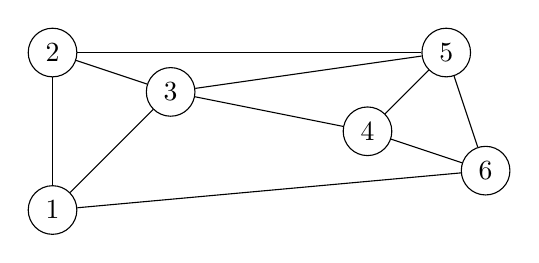
\begin{tikzpicture}
            \node [circle, draw] (1) at (0,0) {1};
            \node [circle, draw] (2) at (0,2) {2};
            \node [circle, draw] (3) at (1.5,1.5) {3};
            \node [circle, draw] (4) at (4,1) {4};
            \node [circle, draw] (5) at (5,2) {5};
            \node [circle, draw] (6) at (5.5,0.5) {6};
            \path [draw] (1) edge (2);
            \path [draw] (2) edge (3);
            \path [draw] (1) edge (3);
            \path [draw] (3) edge (4);
            \path [draw] (4) edge (6);
            \path [draw] (1) edge (6);
            \path [draw] (3) edge (5);
            \path [draw] (4) edge (5);
            \path [draw] (5) edge (6);
            \path [draw] (2) edge (5);
        \end{tikzpicture}
    \end{center}
    Sometimes planarity can be non-obvious (both of the following graphs are equivalent, and are both planar):
    \begin{center}
        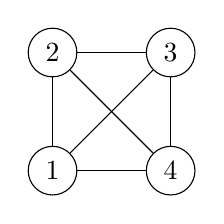
\begin{tikzpicture}
            \node [circle, draw] (1) at (0,0) {1};
            \node [circle, draw] (2) at (0,1.5) {2};
            \node [circle, draw] (3) at (1.5,1.5) {3};
            \node [circle, draw] (4) at (1.5,0) {4};
            \path [draw] (1) edge (2);
            \path [draw] (2) edge (3);
            \path [draw] (3) edge (4);
            \path [draw] (4) edge (1);
            \path [draw] (1) edge (3);
            \path [draw] (2) edge (4);
        \end{tikzpicture}
        \begin{tikzpicture}
            \node [opacity=0] (1) at (0,0) {1};
            \node [opacity=0] (2) at (0,1.5) {2};
            \path [->, thick, draw] (0, 0.8) -- (1, 0.8);
        \end{tikzpicture}
        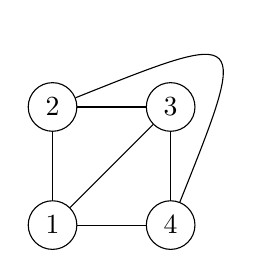
\begin{tikzpicture}
            \node [circle, draw] (1) at (0,0) {1};
            \node [circle, draw] (2) at (0,1.5) {2};
            \node [circle, draw] (3) at (1.5,1.5) {3};
            \node [circle, draw] (4) at (1.5,0) {4};
            \node [opacity=0] (5) at (2,2) {5};
            \path [draw] (1) edge (2);
            \path [draw] (2) edge (3);
            \path [draw] (3) edge (4);
            \path [draw] (4) edge (1);
            \path [draw] (1) edge (3);
            \path [draw] (2) .. controls + (2.5, 1) .. (4);
        \end{tikzpicture}
    \end{center}
\end{frame}

\begin{frame}
    \frametitle{Planar Graphs (Cont.)}
    Here is some planar graph vocabulary:
    \begin{itemize}
        \item {\bf Faces}: Separated regions in our 2D embedding (ex: $6$ faces in first example on previous slide)\\
        \item {\bf Euler's Formula}: $\text{Planar and connected}\implies|V|+|F|=|E|+2$\\
        \item {\bf Euler's Edge Formula}: $\text{Planar and }|V|\geq 3\implies |E|\leq 3|V|-6$\\
        \item {\bf Four-Color Theorem}: $\text{Planar}\implies4\text{-colorable (vertex coloring)}$\\
        \item {\bf Kuratowski's Theorem}: $\text{Planar}\iff\text{No }K_{3,3}\text{ or }K_5\text{ exists}$
        \begin{itemize}
            \item A $K_{m,n}$ is a {\bf complete, bipartite graph} with $m$ vertices in one group and $n$ vertices in the other group, and a $K_n$ is a {\bf complete graph} with $n$ vertices.
        \end{itemize}
    \end{itemize}
\end{frame}

\begin{frame}
    \frametitle{Hypercubes}
    These are $n$-dimensional cubes. Examples of $n=1$, $n=2$, and $n=3$, respectively:\\
    \includegraphics[scale=0.3]{Images/hypercubes.png}\\
    Here is a useful non-geometric interpretation:
    \begin{itemize}
        \item View each node as a bitstring of $n$ bits (there are $2^n$ nodes in an $n$-dimensional hypercube)
        \item An edge between vertex $u$ and vertex $v$ exists iff $u$ and $v$'s bitstring labels differ by exactly one bit
        \item To construct $n+1$-dimensional hypercube with $n$-dimensional hypercubes $A$ and $B$: prepend $1$s to all vertices in $A$, prepend $0$s to all vertices in $B$, and add edges connecting previously identical pairs of vertices in $A$ and $B$
    \end{itemize}
\end{frame}

\begin{frame}
    \frametitle{Hamiltonian Walks/Tours}
    {\bf Hamiltonian Walk}: A walk that visits every vertex in the graph exactly once\\
    {\bf Hamiltonian Tour}: A tour that visits every vertex in the graph exactly once (except starting vertex: visited once at start and once at end)\\
    {\it Note: There is no efficient algorithm to find a Hamiltonian walk/tour in a graph}
\end{frame}

\end{document}